\documentclass[10pt,a4papper]{article}
\usepackage{graphicx}
\usepackage{amsmath}
\usepackage{amssymb}
\usepackage{cancel}
\usepackage{multicol}
\usepackage{blindtext}
\usepackage[hidelinks]{hyperref}
\usepackage[left=2.00cm, right=3.00cm, top=2.00cm, bottom=2.00cm]{geometry}
\setlength{\parindent}{0cm}
\author{Angel Fdo. García Núñez}
\date{Enero 18, 2023}
\title{Estadisitica}

\begin{document}

\Huge
\textbf{Introduction to}\\
\textbf{Quantum Mechanics}\\

\large
\textbf{Second Edition}\\\\\\\\\\\\\\\\

\textbf{David J. Griffiths}\\\\\\\\\\\\\\\\\\\\

\Large
\textbf{Solucionario}\\\\
\large
\textbf{Angel Fernando García Núñez}

\Large
\newpage
\textbf{Problem 1.1} For the distribution of ages in Section 1.3.1:\\

\textbf{(a)} Compute $\langle j^2\rangle$ and $\langle j\rangle^2$.\\
\textbf{(b)} Determine $\Delta j$ for each $j$, and use Equation $1.11$ to compute the standard
deviation.\\
\textbf{(c)} Use your results in (a) and (b) to check Equation $1.12$.

\newpage
\[\text{Valor promedio de }j\]

\[\langle j\rangle=\frac{\sum_{j=0}^\infty jN(j)}{N}=\sum_{j=0}^\infty jP(j)\]

\[N=\sum_{j=0}^\infty N(j)\]

\[N(14)=1\]
\[N(15)=1\]
\[N(16)=3\]
\[N(22)=2\]
\[N(24)=2\]
\[N(25)=5\]

\[N=14\]

\[\langle j\rangle=\frac{14(1)+15(1)+16(3)+22(2)+24(2)+25(5)}{14}=21\]\\

\[\boxed{\textbf{1.1 (a)}\quad\langle j\rangle^2=441}\]\\

\[\text{Valor promedio de }j^2\]

\[\langle j\rangle=\frac{\sum_{j=0}^\infty j^2N(j)}{N}=\sum_{j=0}^\infty j^2P(j)\]

\[\langle j\rangle=\frac{14^2(1)+15^2(1)+16^2(3)+22^2(2)+24^2(2)+25^2(5)}{14}=21\]\\

\[\boxed{\textbf{1.1 (a)}\quad\langle j^2\rangle\approx 459.571}\]

\newpage
\[\text{Desviación de la media}\]

\[\Delta j=j-\langle j\rangle\]

\[j=14\quad\to\quad\Delta j=14-21=-7\]
\[j=15\quad\to\quad\Delta j=15-21=-6\]
\[j=16\quad\to\quad\Delta j=16-21=-5\]
\[j=22\quad\to\quad\Delta j=22-21=1\]
\[j=24\quad\to\quad\Delta j=24-21=3\]
\[j=25\quad\to\quad\Delta j=25-21=4\]

\[\text{Ecuación 1.11 (Definición de varianza)}\]

\[\sigma^2\equiv\langle(\Delta j)^2\rangle\]\\

\[\sigma^2=\frac{\sum_{j=0}^\infty(\Delta j)^2N(j)}{N}\]

\[\sigma^2=\frac{(-7)^2(1)+(-6)^2(1)+(-5)^2(3)+1^2(2)+3^2(2)+4^2(5)}{14}=21\]

\[\boxed{\sigma^2\approx 18.571}\]\\

\[\text{Desviación estándar}\]

\[\sigma=\sqrt{\sigma^2}\]

\[\sigma\approx\sqrt{18.571}\]

\[\boxed{\textbf{1.1 (b)}\quad\sigma\approx 4.309}\]

\newpage
\[\text{Ecuación 1.12}\]

\[\sigma=\sqrt{\langle j^2\rangle-\langle j\rangle^2}\]\\

\[\sigma\approx\sqrt{459.571-441}=\sqrt{18.571}\]\\

\[\text{El resultado en (c) coincide con el resultado en (b)}\]

\[\boxed{\textbf{1.1 (c)}\quad\sigma\approx 4.309}\]

\newpage
\textbf{Problem 1.2}\\

\textbf{(a)} Find the standard deviation of the Example 1.1.\\
\textbf{(b)} What is the probability that a photograph, selected at random, would
show a distance $x$ more than one standard deviation away from average?

\newpage
\[\text{Función de densidad de probabilidad}\]

\[\rho(x)=\frac{1}{2\sqrt{hx}}\quad:\quad x\in(0,h]\]\\

\[\text{Valor de expectación de }x\]

\[\langle x\rangle=\int_{-\infty}^\infty x\rho(x)dx\]\\

\[\langle x\rangle=
\int_0^h x\rho(x)dx=
\int_0^h\frac{x}{2\sqrt{hx}}dx=
\frac{1}{2\sqrt{h}}\int_0^h x^\frac{1}{2}dx=
\frac{1}{2\sqrt{h}}\left|\frac{2}{3}x^\frac{3}{2}\right|_0^h=
\frac{1}{3\sqrt{h}}\left|x^\frac{3}{2}\right|_0^h\]

\[\langle x\rangle=\frac{1}{3\sqrt{h}}\left(h^\frac{3}{2}-0\right)\]

\[\boxed{\langle x\rangle=\frac{h}{3}}\]\\

\[\text{Valor de expectación de }x^2\]

\[\langle x^2\rangle=\int_{-\infty}^\infty x^2\rho(x)dx\]\\

\[\langle x^2\rangle=
\int_0^h x^2\rho(x)dx=
\int_0^h\frac{x^2}{2\sqrt{hx}}dx=
\frac{1}{2\sqrt{h}}\int_0^h x^\frac{3}{2}dx=
\frac{1}{2\sqrt{h}}\left|\frac{2}{5}x^\frac{5}{2}\right|_0^h=
\frac{1}{5\sqrt{h}}\left|x^\frac{5}{2}\right|_0^h\]

\[\langle x^2\rangle=\frac{1}{5\sqrt{h}}\left(h^\frac{5}{2}-0\right)\]

\[\boxed{\langle x^2\rangle=\frac{h^2}{5}}\]

\newpage
\[\text{Desviación estándar}\]

\[\sigma=\sqrt{\langle x^2\rangle-\langle x\rangle^2}\]

\[\sigma=
\sqrt{\frac{h^2}{5}-\left(\frac{h}{3}\right)^2}=
\sqrt{\frac{h^2}{5}-\frac{h^2}{9}}=
\sqrt{\frac{4h^2}{45}}\]\\

\[\boxed{\textbf{1.2 (a)}\quad\sigma=\frac{2h}{3\sqrt{5}}}\]\\

\[\text{Probabilidad de encontrar $x$ fuera de la desviación estándar}\]

\[P=1-\int_{\langle x\rangle-\sigma}^{\langle x\rangle+\sigma}\rho(x)dx\]\\

\[P=
1-\int_{\langle x\rangle-\sigma}^{\langle x\rangle+\sigma}\frac{1}{2\sqrt{hx}}dx=
1-\frac{1}{2\sqrt{h}}\int_{\langle x\rangle-\sigma}^{\langle x\rangle+\sigma}x^{-\frac{1}{2}}dx=
1-\frac{1}{\sqrt{h}}\left|x^{\frac{1}{2}}\right|_{\langle x\rangle-\sigma}^{\langle x\rangle+\sigma}\]

\[P=
1-\frac{1}{\sqrt{h}}\left|x^{\frac{1}{2}}\right|_{\langle x\rangle-\sigma}^{\langle x\rangle+\sigma}=
1-\frac{1}{\sqrt{h}}\left[(\langle x\rangle+\sigma)^{\frac{1}{2}}-(\langle x\rangle-\sigma)^{\frac{1}{2}}\right]\]

\[P=1-\frac{1}{\sqrt{h}}\left[\left(\frac{h}{3}+\frac{2h}{3\sqrt{5}}\right)^{\frac{1}{2}}-\left(\frac{h}{3}-\frac{2h}{3\sqrt{5}}\right)^{\frac{1}{2}}\right]\]\\

\[P\approx 1-\frac{1}{\sqrt{h}}\left[(0.6315h)^\frac{1}{2}-(0.03519h)^\frac{1}{2}\right]=1-0.607\]\\

\[\boxed{\textbf{1.2 (b)}\quad P\approx 0.393}\]

\newpage
\textbf{Problem 1.3} Consider the \textbf{gaussian} distribution\\

\[\rho(x)=Ae^{-\lambda(x-a)^2},\]

where $A$, $a$, and $\lambda$ are real positive constants. (Look up any integrals you
need.)\\

\textbf{(a)} Use Equation 1.16 to determinate $A$.\\
\textbf{(b)} Find $\langle x\rangle$, $\langle x^2\rangle$, and $\sigma$.\\
\textbf{(c)} Sketch the graph of $\rho(x)$.

\newpage
\[\text{Ecuación 1.16}\]

\[\int_{-\infty}^\infty\rho(x)dx=1\]\\

\[\int_{-\infty}^\infty\rho(x)dx=A\int_{-\infty}^\infty e^{-\lambda(x-a)^2}dx=1\]\\

\[\text{Función simétrica}\]

\[\int_{-\infty}^0 e^{-\lambda(x-a)^2}dx=\int_0^\infty e^{-\lambda(x-a)^2}dx\]\\

\[\therefore\quad\int_{-\infty}^\infty\rho(x)dx=2A\int_0^\infty e^{-\lambda(x-a)^2}dx=1\]

\[x=\sqrt{\frac{u}{\lambda}}+a\quad\to\quad u=\lambda(x-a)^2\quad\to\quad du=2\lambda(x-a)dx\quad\to\quad dx=\frac{1}{2\lambda(x-a)}du\]

\[dx=\frac{1}{2\sqrt{\lambda u}}du\]

\[\therefore\quad\int_{-\infty}^\infty\rho(x)dx=\frac{A}{\sqrt{\lambda}}\int_0^\infty u^{-\frac{1}{2}}e^{-u}du=1\]\\

\[\frac{A}{\sqrt{\lambda}}\int_0^\infty u^{-\frac{1}{2}}e^{-u}du=
\frac{A}{\sqrt{\lambda}}\Gamma\left(\frac{1}{2}\right)=
\frac{A}{\sqrt{\lambda}}\sqrt{\pi}=1\]\\

\[\boxed{\textbf{1.3 (a)}\quad A=\sqrt{\frac{\lambda}{\pi}}}\]

\newpage
\[\text{Valor de expectación de }x\]

\[\langle x\rangle=
\int_{-\infty}^\infty x\rho(x)dx=
A\int_{-\infty}^\infty xe^{-\lambda(x-a)^2}dx\]\\

\[u=x-a\quad\to\quad du=dx\]

\[\langle x\rangle=
A\int_{-\infty}^\infty (u+a)e^{-\lambda u^2}du=
A\left[\int_{-\infty}^\infty ue^{-\lambda u^2}du+a\int_{-\infty}^\infty e^{-\lambda u^2}du\right]\]\\

\[\text{Función impar}\]

\[\int_{-\infty}^0 ue^{-\lambda u^2}du=-\int_0^\infty ue^{-\lambda u^2}du\quad\to\quad
\int_{-\infty}^\infty ue^{-\lambda u^2}du=0\]

\[\text{Función par}\]

\[\int_{-\infty}^0 e^{-\lambda u^2}du=\int_0^\infty e^{-\lambda u^2}du\quad\to\quad
\int_{-\infty}^\infty e^{-\lambda u^2}du=2\int_0^\infty e^{-\lambda u^2}du\]\\

\[\therefore\quad\langle x\rangle=2aA\int_0^\infty e^{-\lambda u^2}du\]

\newpage
\[u=\sqrt{\frac{t}{\lambda}}\quad\to\quad t=\lambda u^2\quad\to\quad dt=2\lambda udu\quad\to\quad du=\frac{1}{2\lambda u}dt\]

\[du=\frac{1}{2\sqrt{\lambda t}}dt\]\\

\[\langle x\rangle=
\frac{aA}{\sqrt{\lambda}}\int_0^\infty t^{-\frac{1}{2}}e^{-t}dt=
\frac{aA}{\sqrt{\lambda}}\Gamma\left(\frac{1}{2}\right)=
\frac{aA}{\sqrt{\lambda}}\sqrt{\pi}\]\\

\[A=\sqrt{\frac{\lambda}{\pi}}\quad\to\quad\langle x\rangle=a\sqrt{\frac{\lambda}{\pi}}\sqrt{\frac{\pi}{\lambda}}\]\\

\[\boxed{\textbf{1.3 (b)}\quad\langle x\rangle=a}\]

\newpage
\[\text{Valor de expectación de }x^2\]

\[\langle x^2\rangle=
\int_{-\infty}^\infty x^2\rho(x)dx=
A\int_{-\infty}^\infty x^2e^{-\lambda(x-a)^2}dx\]\\

\[u=x-a\quad\to\quad du=dx\]

\[\langle x^2\rangle=
A\int_{-\infty}^\infty (u+a)^2e^{-\lambda u^2}du=
A\left[\int_{-\infty}^\infty u^2e^{-\lambda u^2}du+a^2\int_{-\infty}^\infty e^{-\lambda u^2}du+2a\int_{-\infty}^\infty ue^{-\lambda u^2}du\right]\]\\

\[\text{Función impar}\]

\[\int_{-\infty}^\infty ue^{-\lambda u^2}du=0\]\\

\[\text{Funciones pares}\]

\[\int_{-\infty}^\infty e^{-\lambda u^2}du=2\int_0^\infty e^{-\lambda u^2}du\quad,\quad
\int_{-\infty}^\infty u^2e^{-\lambda u^2}du=2\int_0^\infty u^2e^{-\lambda u^2}du\]\\

\[\langle x^2\rangle=A\left[2\int_0^\infty u^2e^{-\lambda u^2}du+2a\int_0^\infty e^{-\lambda u^2}du\right]\]

\newpage
\[u=\sqrt{\frac{t}{\lambda}}\quad\to\quad t=\lambda u^2\quad\to\quad dt=2\lambda udu\quad\to\quad du=\frac{1}{2\lambda u}dt\]

\[du=\frac{1}{2\sqrt{\lambda t}}dt\]

\[\langle x^2\rangle=
\frac{A}{\sqrt{\lambda}}\left[
  \int_0^\infty\left(\frac{t}{\lambda}\right)t^{-\frac{1}{2}}e^{-t}dt
  +a^2\int_0^\infty t^{-\frac{1}{2}}e^{-t}dt\right]\]\\

\[\langle x^2\rangle=
\frac{A}{\sqrt{\lambda}}\left[
  \frac{1}{\lambda}\int_0^\infty t^\frac{1}{2}e^{-t}dt
  +a^2\int_0^\infty t^{-\frac{1}{2}}e^{-t}dt\right]=
\frac{A}{\sqrt{\lambda}}\left[\frac{1}{\lambda}\Gamma\left(\frac{3}{2}\right)+a^2\Gamma\left(\frac{1}{2}\right)\right]\]\\

\[\langle x^2\rangle=
\frac{A}{\sqrt{\lambda}}\left[\frac{\sqrt{\pi}}{2\lambda}+a^2\sqrt{\pi}\right]\]\\

\[A=\sqrt{\frac{\lambda}{\pi}}\quad\to\quad
\langle x^2\rangle=
\frac{\sqrt{\frac{\lambda}{\pi}}}{\sqrt{\lambda}}\left[\frac{\sqrt{\pi}}{2\lambda}+a^2\sqrt{\pi}\right]=
\frac{1}{2\lambda}+a^2\]\\

\[\boxed{\textbf{1.3 (b)}\quad\langle x^2\rangle=a^2+\frac{1}{2\lambda}}\]\\

\[\text{Desviación estándar}\]

\[\sigma=
\sqrt{\langle x^2\rangle-\langle x\rangle^2}=
\sqrt{\left(a^2+\frac{1}{2\lambda}\right)-a^2}\]\\

\[\boxed{\textbf{1.3 (b)}\quad\sigma=\frac{1}{\sqrt{2\lambda}}}\]

\newpage
\[\text{Función de densidad de probabilidad}\]

\[\rho(x)=Ae^{-\lambda(x-a)^2}\]

\[\boxed{\textbf{1.3 (c)}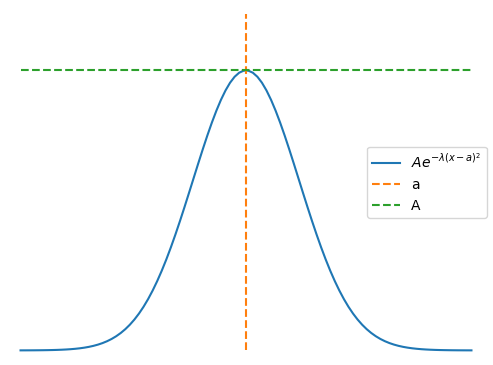
\includegraphics[width=8cm]{p1.3c.png}}\]

\newpage
\textbf{Problem 1.4} At time $t=0$ a particle is represented by the wave function

\[\Psi(x,0)=
\left\{\begin{array}{lll}
A\frac{x}{a}, & & \text{if } 0\leq x\leq a,\\
A\frac{(b-x)}{(b-a)}, & & \text{if } a\leq x\leq b,\\
0, & & \text{otherwise},
\end{array}\]\\

where $A$, $a$, and $b$ are constansts.\\\\
\textbf{(a)} Normalize $\Psi$ (that is, find $A$, in termis of $a$ and $b$).\\
\textbf{(b)} Sketch $\Psi(x,0)$. as a function of $x$.\\
\textbf{(c)} Where is the particle most likely to be found, at $t=0$?\\
\textbf{(d)} What is the probability of finding the particle to the left of $a$? Check your results in the limiting cases $b=a$ and $b=2a$.\\
\textbf{(e)} What is the expectation value of $x$?

\newpage
\[\text{Función de onda en }t=0\]

\[\Psi(x,0)=
\left\{\begin{array}{lll}
A\frac{x}{a} & : & 0\leq x\leq a\\
A\frac{(b-x)}{(b-a)} & : & a\leq x\leq b\\
0 & : & x<0 \vee x>b
\end{array}\]\\

\[\text{Función de densidad}\]

\[|\Psi(x,0)|^2=
\left\{\begin{array}{lll}
A^2\frac{x^2}{a^2} & : & 0\leq x\leq a\\
A^2\frac{(b-x)^2}{(b-a)^2} & : & a\leq x\leq b\\
0 & : & x<0 \vee x>b
\end{array}\]\\

\[\text{Normalización}\]

\[\int_{-\infty}^\infty|\Psi(x,0)|^2dx=1\]

\[\cancelto{0}{\int_{-\infty}^0|\Psi(x,0)|^2dx}+\int_0^a|\Psi(x,0)|^2dx+\int_a^b|\Psi(x,0)|^2dx+\cancelto{0}{\int_b^\infty|\Psi(x,0)|^2dx}=1\]\\

\[\frac{A^2}{a^2}\int_0^ax^2dx+\frac{A^2}{(b-a)^2}\int_a^b(b-x)^2dx=1\]\\

\[u(x)=b-x\quad\to\quad du=-dx\]

\[u(a)=b-a\quad,\quad u(b)=0\]

\[\frac{A^2}{a^2}\int_0^ax^2dx-\frac{A^2}{(b-a)^2}\int_{b-a}^0u^2du=1\]

\newpage
\[\frac{A^2}{a^2}\left|\frac{x^3}{3}\right|_0^a-\frac{A^2}{(b-a)^2}\left|\frac{u^3}{3}\right|_{b-a}^0=
\frac{A^2}{a^2}\left(\frac{a^3}{3}\right)+\frac{A^2}{(b-a)^2}\left[\frac{(b-a)^3}{3}\right]=1\]\\

\[\frac{A^2}{3}[a+(b-a)]=1\quad\to\quad\frac{b}{3}A^2=1\]

\[\boxed{\textbf{1.4 (a)}\quad A=\sqrt{\frac{3}{b}}}\]\\\\

\[\text{Bosquejo de }\Psi(x,0)\]

\[\boxed{\textbf{1.4 (b)}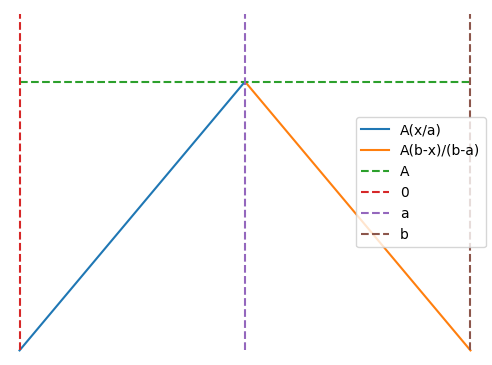
\includegraphics[width=8cm]{p1.4b.png}}\]

\newpage
\[\text{Bosquejo de }|\Psi(x,0)|^2\]

\[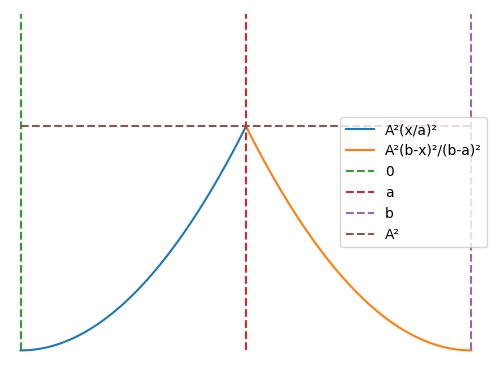
\includegraphics[width=8cm]{p1.4c.png}\]

Como se puede ver en el boceto de la función de densidad $|\Psi(x,0)|^2$, el
valor máximo y la posición donde es mas probable que se encuentre la partícula es
en $x=a$, con una probabilidad de $P(x=a)=|\Psi(a,0)|^2=A^2=\frac{3}{b}$.

\[\boxed{\textbf{1.4 (c)}\quad x=a}\]

\newpage
\[\text{Probabilidad de la posición de la partícula en un intervalo}\]

\[P(a\leq x\leq b)=\int_a^b|\Psi(x,t)|^2dx=\int_a^b|\Psi(x,0)|^2dx\]\\

\[\text{Probabilidad a la izquierda de }a\]

\[P(x\leq a)=\int_{-\infty}^a|\Psi(x,t)|^2dx=\int_{-\infty}^a|\Psi(x,0)|^2dx\]

\[P(x\leq a)=
\cancelto{0}{\int_{-\infty}^0|\Psi(x,0)|^2dx}+\int_0^a|\Psi(x,0)|^2dx=
\frac{A^2}{a^2}\int_0^ax^2dx\]

\[P(x\leq a)=
\frac{A^2}{a^2}\left|\frac{x^3}{3}\right|_0^a=
\frac{A^2}{a^2}\left(\frac{a^3}{3}\right)=
\frac{a}{3}A^2\]

\[A^2=\frac{3}{b}\quad\to\quad P(x\leq a)=\frac{a}{3}\left(\frac{3}{b}\right)\]\\

\[\boxed{\therefore\quad P(x\leq a)=\frac{a}{b}}\]\\

\[\text{Caso }b=a\]

\[\boxed{\textbf{1.4 (d)}\quad P(x\leq a)=1}\]\\

\[\text{Caso }b=2a\]

\[\boxed{\textbf{1.4 (d)}\quad P(x\leq a)=\frac{1}{2}}\]

\newpage
\[\text{Valor de expectación de }x\]

\[\langle x\rangle=\int_{-\infty}^\infty x|\Psi(x,0)|^2dx\]

\[\langle x\rangle=\int_0^a x|\Psi(x,0)|^2dx+\int_a^b x|\Psi(x,0)|^2dx\]\\

\[\langle x\rangle=\frac{A^2}{a^2}\int_0^a x^3dx+\frac{A^2}{(b-a)^2}\int_a^b x(b-x)^2dx\]

\[\langle x\rangle=\frac{A^2}{a^2}\int_0^a x^3dx+\frac{A^2}{(b-a)^2}\int_a^b x(x^2-2bx+b^2)dx\]

\[\langle x\rangle=\frac{A^2}{a^2}\int_0^a x^3dx+\frac{A^2}{(b-a)^2}\int_a^b (x^3-2bx^2+b^2x)dx\]\\

\[\langle x\rangle=
\frac{A^2}{a^2}\int_0^a x^3dx
+\frac{A^2}{(b-a)^2}\int_a^b x^3dx
-\frac{2bA^2}{(b-a)^2}\int_a^b x^2dx
+\frac{b^2A^2}{(b-a)^2}\int_a^b xdx\]\\

\[\langle x\rangle=
\frac{A^2}{a^2}\left|\frac{x^4}{4}\right|_0^a
+\frac{A^2}{(b-a)^2}\left|\frac{x^4}{4}\right|_a^b
-\frac{2bA^2}{(b-a)^2}\left|\frac{x^3}{3}\right|_a^b
+\frac{b^2A^2}{(b-a)^2}\left|\frac{x^2}{2}\right|_a^b\]\\

\[\langle x\rangle=
\frac{A^2}{a^2}\left(\frac{a^4}{4}\right)
+\frac{A^2}{(b-a)^2}\left(\frac{b^4}{4}-\frac{a^4}{4}\right)
-\frac{2bA^2}{(b-a)^2}\left(\frac{b^3}{3}-\frac{a^3}{3}\right)
+\frac{b^2A^2}{(b-a)^2}\left(\frac{b^2}{2}-\frac{a^2}{2}\right)\]\\

\[\langle x\rangle=
\left[\frac{1}{4}a^2
+\frac{(b^4-a^4)}{4(b-a)^2}
-\frac{2b(b^3-a^3)}{3(b-a)^2}
+\frac{b^2(b^2-a^2)}{2(b-a)^2}\right]A^2\]

\newpage
\[A^2=\frac{3}{b}\]

\[\langle x\rangle=
\frac{3}{b}
\left[\frac{1}{4}a^2
+\frac{(b^4-a^4)}{4(b-a)^2}
-\frac{2b(b^3-a^3)}{3(b-a)^2}
+\frac{b^2(b^2-a^2)}{2(b-a)^2}\right]\]\\

\[\langle x\rangle=
\frac{3}{4b(b-a)^2}
\left[a^2(b-a)^2
+(b^4-a^4)
-\frac{8}{3}b(b^3-a^3)
+2b^2(b^2-a^2)\right]\]\\

\[\langle x\rangle=
\frac{3}{4b(b-a)^2}
\left[a^2(a^2+b^2-2ab)
+(b^4-a^4)
-\frac{8}{3}(b^4-a^3b)
+2(b^4-a^2b^2)\right]\]\\

\[\langle x\rangle=
\frac{3}{4b(b-a)^2}
\left[(a^4+a^2b^2-2a^3b)
+(b^4-a^4)
-\frac{8}{3}(b^4-a^3b)
+2(b^4-a^2b^2)\right]\]\\

\[\langle x\rangle=
\frac{3}{4b(b-a)^2}\left(\frac{2}{3}a^3b+\frac{1}{3}b^4-a^2b^2\right)=
\frac{2a^3+b^3-3a^2b}{4(b-a)^2}=
\frac{(2a+b)(a^2+b^2-2ab)}{4(b-a)^2}\]\\

\[\langle x\rangle=\frac{(2a+b)(b-a)^2}{4(b-a)^2}\]\\

\[\boxed{\textbf{1.4 (e)}\quad\langle x\rangle=\frac{2a+b}{4}}\]

\newpage
\textbf{Problem 1.5} Consider the wave function

\[\Psi(x,t)=Ae^{-\lambda|x|}e^{-i\omega t}\]

where $A$, $\lambda$, and $\omega$ are positive real constans. (We'll see in Chapter 2 what
potential ($V$) actually produces such a wave function.)\\

\textbf{(a)} Normalize $\Psi$.\\
\textbf{(b)} Determine the exprectation values of $x$ and $x^2$.\\
\textbf{(c)} Find the standard deviation of $x$. Sketch the graph of $|\Psi|^2$, as a function
of $x$, and mark the points $(\langle x\rangle+\sigma)$ and $(\langle x\rangle-\sigma)$, to illustrate the sense in
which $\sigma$ represents the ``spread'' in $x$. What is the probability that the
particle would be found outside this range?

\newpage
\[\text{Función de onda}\]

\[\Psi(x,t)=
Ae^{-\lambda|x|}e^{-i\omega t}=
\left\{\begin{array}{lll}
Ae^{\lambda x}e^{-i\omega t} & : & x\leq 0\\
Ae^{-\lambda x}e^{-i\omega t} & : & x>0
\end{array}\]\\

\[\text{Función de densidad}\]

\[|\Psi(x,t)|^2=
A^2e^{-2\lambda|x|}=
\left\{\begin{array}{lll}
A^2e^{2\lambda x} & : & x\leq 0\\
A^2e^{-2\lambda x} & : & x>0
\end{array}\]\\

\[\text{Normalización}\]

\[\int_{-\infty}^\infty|\Psi(x,t)|^2dx=1\]\\

\[\int_{-\infty}^\infty|\Psi(x,t)|^2dx=
\int_{-\infty}^0|\Psi(x,t)|^2dx+\int_0^\infty|\Psi(x,t)|^2dx=1\]

\[A^2\int_{-\infty}^0 e^{2\lambda x}dx+A^2\int_0^\infty e^{-2\lambda x}dx=1\quad\to\quad
A^2\left|\frac{e^{2\lambda x}}{2\lambda}\right|_{-\infty}^0-A^2\left|\frac{e^{-2\lambda x}}{2\lambda}\right|_0^\infty=1\]

\[\frac{A^2}{2\lambda}\left[
  \left(\cancelto{1}{e^{0}}-\cancelto{0}{\lim_{x\to-\infty}e^{2\lambda x}}\right)
  -\left(\cancelto{0}{\lim_{x\to\infty}e^{-2\lambda x}}-\cancelto{1}{e^{0}}\right)\right]=1\quad\to\quad
\frac{A^2}{\lambda}=1\]\\

\[\boxed{\therefore\quad A=\sqrt{\lambda}}\]\\

\[\boxed{\textbf{1.5 (a)}\quad\Psi(x,t)=\sqrt{\lambda}e^{-\lambda|x|}e^{-i\omega t}}\]

\newpage
\[\text{Valor de expectación de }x\]

\[\langle x\rangle=\int_{-\infty}^\infty x|\Psi(x,t)|^2dx\]\\

\[\langle x\rangle=\lambda\int_{-\infty}^0 xe^{2\lambda x}dx+\lambda\int_0^\infty xe^{-2\lambda x}dx\]\\

\[\text{Función impar}\]

\[\int_{-\infty}^0 xe^{2\lambda x}dx=-\int_0^\infty xe^{-2\lambda x}dx\]\\

\[\therefore\quad\langle x\rangle=-\lambda\int_0^\infty xe^{-2\lambda x}dx+\lambda\int_0^\infty xe^{-2\lambda x}dx\]\\

\[\boxed{\textbf{1.5 (b)}\quad\langle x\rangle=0}\]

\newpage
\[\text{Valor de expectación de }x^2\]

\[\langle x^2\rangle=\int_{-\infty}^\infty x^2|\Psi(x,t)|^2dx\]\\

\[\langle x^2\rangle=\lambda\int_{-\infty}^0 x^2e^{2\lambda x}dx+\lambda\int_0^\infty x^2e^{-2\lambda x}dx\]\\

\[\text{Función par}\]

\[\int_{-\infty}^0 x^2e^{2\lambda x}dx=\int_0^\infty x^2e^{-2\lambda x}dx\]\\

\[\therefore\quad\langle x^2\rangle=2\lambda\int_0^\infty x^2e^{-2\lambda x}dx\]\\

\[x=\frac{1}{2\lambda}t\quad\to\quad t=2\lambda x\quad\to\quad dt=2\lambda dx\quad\to\quad dx=\frac{1}{2\lambda}dt\]\\

\[\langle x^2\rangle=
2\lambda\int_0^\infty\left(\frac{1}{2\lambda}t\right)^2e^{-t}\left(\frac{1}{2\lambda}dt\right)=
\frac{1}{4\lambda^2}\int_0^\infty t^2e^{-t}dt\]

\newpage
\[\text{Función Gamma}\]

\[\Gamma(x)=\int_0^\infty t^{x-1}e^{-t}dt\]\\

\[\langle x^2\rangle=
\frac{1}{4\lambda^2}\int_0^\infty t^{3-1}e^{-t}dt=
\frac{1}{4\lambda^2}\Gamma(3)=
\frac{(3-1)!}{4\lambda^2}=
\frac{2!}{4\lambda^2}\]\\

\[\boxed{\textbf{1.5 (b)}\quad\langle x^2\rangle=\frac{1}{2\lambda^2}}\]\\

\[\text{Desviación estándar}\]

\[\sigma=
\sqrt{\langle x^2\rangle-\langle x\rangle^2}=
\sqrt{\frac{1}{2\lambda^2}-0}\]

\[\boxed{\textbf{1.5 (c)}\quad\sigma=\frac{1}{\sqrt{2}\lambda}}\]\\

\[\text{Bosquejo de }|\Psi(x,t)|^2=A^2e^{-2\lambda|x|}\]
\[\boxed{\textbf{1.5 (c)}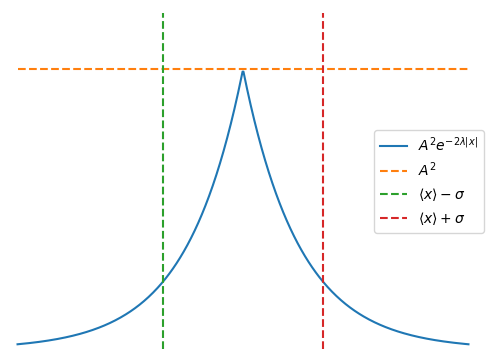
\includegraphics[width=8cm]{p1.5c.png}}\]

\newpage
\[\text{Probabilidad de la posición de la partícula fuera de un intervalo}\]

\[P(x<a\vee x>b)=\int_{-\infty}^a|\Psi(x,t)|^2dx+\int_b^\infty|\Psi(x,t)|^2dx\]\\

\[\text{Probabilidad fuera de la desviación estándar}\]

\[P=\int_{-\infty}^a|\Psi(x,t)|^2dx+\int_b^\infty|\Psi(x,t)|^2dx\]\\

\[P=
\int_{-\infty}^{\langle x\rangle-\sigma}|\Psi(x,t)|^2dx+\int_{\langle x\rangle+\sigma}^\infty|\Psi(x,t)|^2dx=
\int_{-\infty}^{-\sigma}|\Psi(x,t)|^2dx+\int_{\sigma}^\infty|\Psi(x,t)|^2dx\]\\

\[P=A^2\int_{-\infty}^{-\sigma}e^{2\lambda x}dx+A^2\int_{\sigma}^\infty e^{-2\lambda x}dx\]\\

\[A^2\int_{-\infty}^{-\sigma}e^{2\lambda x}dx=A^2\int_{\sigma}^\infty e^{-2\lambda x}dx\quad\to\quad
P=2A^2\int_{\sigma}^\infty e^{-2\lambda x}dx\]

\[A^2=\lambda\quad\to\quad P=2\lambda\int_{\sigma}^\infty e^{-2\lambda x}dx\]\\

\[P=
-\left|e^{-2\lambda x}\right|_{\sigma}^\infty=
e^{-2\lambda\sigma}-\cancelto{0}{\lim_{x\to\infty}e^{-2\lambda x}}=
e^{-2\lambda\sigma}\]

\[\sigma=\frac{1}{\sqrt{2}\lambda}\quad\to\quad
P=
e^{-2\lambda\left(\frac{1}{\sqrt{2}\lambda}\right)}=
e^{-\sqrt{2}}\]

\[\boxed{\textbf{1.5 (c)}\quad P\approx 0.2431}\]

\newpage
\textbf{Problem 1.6} Why can't you do integration-by-parts directly on the middle
expression in Equation 1.29---pull the time derivative over onto $x$, note that
$\partial x/\partial t=0$, and conclude that $d\langle x\rangle/dt=0$?

\newpage
\[\text{Ecuación 1.29}\]

\[\frac{d\langle x\rangle}{dt}=
\int x\frac{\partial}{\partial t}|\Psi|^2dx=
\frac{i\hbar}{2m}\int x\frac{\partial}{\partial x}\left(\bar\Psi\frac{\partial\Psi}{\partial x}-\Psi\frac{\partial\bar\Psi}{\partial x}\right)dx\]\\

\fbox{\begin{minipage}{17cm}
    No se puede recurrir a integración por partes, ya que para ello la variable
    de diferenciación e integración deben ser la misma, cosa que no ocurre en la
    expresión del medio en la ecuación 1.29.
\end{minipage}}\\\\

\[\frac{\partial x}{\partial t}=0\quad\to\quad
x\frac{\partial}{\partial t}|\Psi|^2=\frac{\partial}{\partial t}\left(x|\Psi|^2\right)\]

\[\therefore\quad\frac{d\langle x\rangle}{dt}=\int\frac{\partial}{\partial t}\left(x|\Psi|^2\right)dx\]\\

\[\rho(x)=|\Psi(x,t)|^2\quad\to\quad
\frac{\partial\rho}{\partial t}=\frac{\partial}{\partial t}|\Psi|^2=0\]\\

\[\therefore\]

\[\boxed{\textbf{1.6}\quad\frac{d\langle x\rangle}{dt}=0}\]

\newpage
\textbf{Problem 1.7} Calculate $d\langle p\rangle/dt$. Answer:

\[\frac{d\langle p\rangle}{dt}=\left\langle-\frac{\partial V}{\partial x}\right\rangle.\]

Equations 1.32 (or the first part of 1.33) and 1.38 are instances of \textbf{Ehrenfest's
  theorem,} which tells us that \emph{expectation values obey classic laws}.

\newpage
\[\text{Ecuación 1.33}\]

\[\langle p\rangle=m\frac{d\langle x\rangle}{dt}=-i\hbar\int\left(\bar\Psi\frac{\partial\Psi}{\partial x}\right)dx\]\\

\[\frac{d\langle p\rangle}{dt}=-i\hbar\int\frac{\partial}{\partial t}\left(\bar\Psi\frac{\partial\Psi}{\partial x}\right)dx\]\\

\[\frac{\partial}{\partial t}\left(\bar\Psi\frac{\partial\Psi}{\partial x}\right)=
\frac{\partial\bar\Psi}{\partial t}\frac{\partial\Psi}{\partial x}+\bar\Psi\frac{\partial^2\Psi}{\partial t\partial x}\]\\

\[\text{Ecuación de Schrödinger}\]

\[\frac{\partial\Psi}{\partial t}=\frac{i\hbar}{2m}\frac{\partial^2\Psi}{\partial x^2}-\frac{i}{\hbar}V\Psi\quad\to\quad
\frac{\partial\bar\Psi}{\partial t}=-\frac{i\hbar}{2m}\frac{\partial^2\bar\Psi}{\partial x^2}+\frac{i}{\hbar}V\bar\Psi\]\\

\[\frac{\partial}{\partial t}\left(\bar\Psi\frac{\partial\Psi}{\partial x}\right)=
\frac{\partial\Psi}{\partial x}\left(-\frac{i\hbar}{2m}\frac{\partial^2\bar\Psi}{\partial x^2}+\frac{i}{\hbar}V\bar\Psi\right)
+\bar\Psi\frac{\partial}{\partial x}\left(\frac{i\hbar}{2m}\frac{\partial^2\Psi}{\partial x^2}-\frac{i}{\hbar}V\Psi\right)\]\\

\[\frac{\partial}{\partial t}\left(\bar\Psi\frac{\partial\Psi}{\partial x}\right)=
\frac{\partial\Psi}{\partial x}\left(-\frac{i\hbar}{2m}\frac{\partial^2\bar\Psi}{\partial x^2}+\frac{i}{\hbar}V\bar\Psi\right)
+\frac{i\hbar}{2m}\bar\Psi\frac{\partial^3\Psi}{\partial x^3}-\frac{i}{\hbar}\bar\Psi\frac{\partial}{\partial x}(V\Psi)\]\\

\[\frac{\partial}{\partial t}\left(\bar\Psi\frac{\partial\Psi}{\partial x}\right)=
\frac{\partial\Psi}{\partial x}\left(-\frac{i\hbar}{2m}\frac{\partial^2\bar\Psi}{\partial x^2}+\frac{i}{\hbar}V\bar\Psi\right)
+\frac{i\hbar}{2m}\bar\Psi\frac{\partial^3\Psi}{\partial x^3}
-\frac{i}{\hbar}V\bar\Psi\frac{\partial\Psi}{\partial x}
-\frac{i}{\hbar}|\Psi|^2\frac{\partial V}{\partial x}\]

\newpage
\[\frac{\partial}{\partial t}\left(\bar\Psi\frac{\partial\Psi}{\partial x}\right)=
-\frac{i\hbar}{2m}\frac{\partial^2\bar\Psi}{\partial x^2}\frac{\partial\Psi}{\partial x}
+\frac{i\hbar}{2m}\bar\Psi\frac{\partial^3\Psi}{\partial x^3}
-\frac{i}{\hbar}|\Psi|^2\frac{\partial V}{\partial x}\]\\

\[\frac{\partial}{\partial t}\left(\bar\Psi\frac{\partial\Psi}{\partial x}\right)=
\frac{i\hbar}{2m}\left[
  \bar\Psi\frac{\partial^3\Psi}{\partial x^3}
  -\frac{\partial^2\bar\Psi}{\partial x^2}\frac{\partial\Psi}{\partial x}\right]
-\frac{i}{\hbar}|\Psi|^2\frac{\partial V}{\partial x}\]\\

\[\therefore\quad\frac{d\langle p\rangle}{dt}=
\frac{\hbar^2}{2m}\int_{-\infty}^\infty\left[
  \bar\Psi\frac{\partial^3\Psi}{\partial x^3}
  -\frac{\partial^2\bar\Psi}{\partial x^2}\frac{\partial\Psi}{\partial x}\right]dx
-\int_{-\infty}^\infty|\Psi|^2\frac{\partial V}{\partial x}dx\]\\

\[\frac{d\langle p\rangle}{dt}=
\frac{\hbar^2}{2m}\left[
  \int_{-\infty}^\infty\bar\Psi\frac{\partial^3\Psi}{\partial x^3}dx
  -\int_{-\infty}^\infty\frac{\partial^2\bar\Psi}{\partial x^2}\frac{\partial\Psi}{\partial x}dx\right]
-\int_{-\infty}^\infty|\Psi|^2\frac{\partial V}{\partial x}dx\]\\

\[u=\frac{\partial\Psi}{\partial x}\quad\to\quad du=\frac{\partial^2\Psi}{\partial x^2}dx\]

\[dv=\frac{\partial^2\bar\Psi}{\partial x^2}dx\quad\to\quad v=\frac{\partial\bar\Psi}{\partial x}\]\\

\[\frac{d\langle p\rangle}{dt}=
\frac{\hbar^2}{2m}\left[
  \int_{-\infty}^\infty\bar\Psi\frac{\partial^3\Psi}{\partial x^3}dx
  -\left|\frac{\partial\bar\Psi}{\partial x}\frac{\partial\Psi}{\partial x}\right|_{-\infty}^\infty
  +\int_{-\infty}^\infty\frac{\partial\bar\Psi}{\partial x}\frac{\partial^2\Psi}{\partial x^2}dx\right]
-\int_{-\infty}^\infty|\Psi|^2\frac{\partial V}{\partial x}dx\]\\

\[\lim_{|x|\to\infty}\frac{\partial\Psi}{\partial x}=\lim_{|x|\to\infty}\frac{\partial\bar\Psi}{\partial x}=0\quad\to\quad
\left|\frac{\partial\bar\Psi}{\partial x}\frac{\partial\Psi}{\partial x}\right|_{-\infty}^\infty=0\]\\

\[\frac{d\langle p\rangle}{dt}=
\frac{\hbar^2}{2m}\left[
  \int_{-\infty}^\infty\bar\Psi\frac{\partial^3\Psi}{\partial x^3}dx
  +\int_{-\infty}^\infty\frac{\partial\bar\Psi}{\partial x}\frac{\partial^2\Psi}{\partial x^2}dx\right]
-\int_{-\infty}^\infty|\Psi|^2\frac{\partial V}{\partial x}dx\]

\newpage
\[u=\frac{\partial^2\Psi}{\partial x^2}\quad\to\quad du=\frac{\partial^3\Psi}{\partial x^3}dx\]

\[dv=\frac{\partial\bar\Psi}{\partial x}dx\quad\to\quad v=\bar\Psi\]\\

\[\frac{d\langle p\rangle}{dt}=
\frac{\hbar^2}{2m}\left[
  \int_{-\infty}^\infty\bar\Psi\frac{\partial^3\Psi}{\partial x^3}dx
  +\left|\bar\Psi\frac{\partial^2\Psi}{\partial x^2}\right|_{-\infty}^\infty
  -\int_{-\infty}^\infty\bar\Psi\frac{\partial^3\Psi}{\partial x^3}dx\right]
-\int_{-\infty}^\infty|\Psi|^2\frac{\partial V}{\partial x}dx\]\\

\[\lim_{|x|\to\infty}\Psi=\lim_{|x|\to\infty}\bar\Psi=0\quad\to\quad
\left|\bar\Psi\frac{\partial^2\Psi}{\partial x^2}\right|_{-\infty}^\infty=0\]\\

\[\therefore\quad\frac{d\langle p\rangle}{dt}=
-\int_{-\infty}^\infty|\Psi|^2\frac{\partial V}{\partial x}dx=
\int_{-\infty}^\infty\bar\Psi\Psi\left(-\frac{\partial V}{\partial x}\right)dx=
\int_{-\infty}^\infty\bar\Psi\left(-\frac{\partial V}{\partial x}\Psi\right)dx\]\\

\[\boxed{\textbf{1.7}\quad\frac{d\langle p\rangle}{dt}=\left\langle-\frac{\partial V}{\partial x}\right\rangle\quad\blacksquare}\]

\newpage
\textbf{Problem 1.8} Supose you add a constant $V_0$ to the potential energy (by
``constant'' I mean independent of $x$ as well as $t$). In classical mechanics this
doesn't change anything, but what about \emph{quantum mechanics}? Show that
the wave function picks up a time-dependent phase factor: exp$(-iV_0/\hbar)$. What
effect does this have on the expectation value of a dynamical variable?

\newpage
\[\text{Ecuación de Schrödinger}\]

\[\hat H\Psi=i\hbar\frac{\partial\Psi}{\partial t}\]

\[-\frac{\hbar^2}{2m}\frac{\partial^2\Psi}{\partial x^2}+V\Psi=i\hbar\frac{\partial\Psi}{\partial t}\]\\

\[-\frac{\hbar^2}{2m}\frac{\partial^2\Phi}{\partial x^2}+(V+V_0)\Phi=i\hbar\frac{\partial\Phi}{\partial t}\]\\

\[\frac{\partial\Phi}{\partial t}+\frac{i}{\hbar}V_0\Phi=\frac{i\hbar}{2m}\frac{\partial^2\Phi}{\partial x^2}-\frac{i}{\hbar}V(x)\Phi\]\\

\[\text{Método de factor integrante}\]

\[\frac{df}{dt}+P(t)f(t)=g(t)\quad\to\quad\mu\frac{df}{dt}+\mu P(t)f(t)=\mu g(t)\]

\[\mu=e^{\int P(t)dt}\]\\

\[\mu\frac{\partial\Phi}{\partial t}+\mu\frac{i}{\hbar}V_0\Phi=\mu\frac{i\hbar}{2m}\frac{\partial^2\Phi}{\partial x^2}-\mu\frac{i}{\hbar}V(x)\Phi\]\\

\[\mu=e^{\int_0^t\frac{i}{\hbar}V_0dt'}=e^{\frac{i}{\hbar}V_0\int_0^tdt'}=e^{\frac{i}{\hbar}V_0t}\]

\[e^{\frac{i}{\hbar}V_0t}\frac{\partial\Phi}{\partial t}+e^{\frac{i}{\hbar}V_0t}\frac{i}{\hbar}V_0\Phi=
e^{\frac{i}{\hbar}V_0t}\frac{i\hbar}{2m}\frac{\partial^2\Phi}{\partial x^2}-e^{\frac{i}{\hbar}V_0t}\frac{i}{\hbar}V(x)\Phi\]

\newpage
\[e^{\frac{i}{\hbar}V_0t}\frac{\partial\Phi}{\partial t}+e^{\frac{i}{\hbar}V_0t}\frac{i}{\hbar}V_0\Phi=
e^{\frac{i}{\hbar}V_0t}\frac{i\hbar}{2m}\frac{\partial^2\Phi}{\partial x^2}-e^{\frac{i}{\hbar}V_0t}\frac{i}{\hbar}V(x)\Phi\]\\

\[\frac{\partial}{\partial t}\left(\Phi e^{\frac{i}{\hbar}V_0t}\right)=
\frac{i\hbar}{2m}\frac{\partial^2}{\partial x^2}\left(\Phi e^{\frac{i}{\hbar}V_0t}\right)-\frac{i}{\hbar}V(x)\left(\Phi e^{\frac{i}{\hbar}V_0t}\right)\]\\

\[\boxed{\Psi(x,t)=\Phi(x,t)e^{\frac{i}{\hbar}V_0t}\quad\to\quad
\Phi(x,t)=\Psi(x,t)e^{-\frac{i}{\hbar}V_0t}}\]\\

\[\frac{\partial\Psi}{\partial t}=\frac{i\hbar}{2m}\frac{\partial^2\Psi}{\partial x^2}-\frac{i}{\hbar}V(x)\Psi\quad\to\quad
-\frac{\hbar^2}{2m}\frac{\partial^2\Psi}{\partial x^2}+V\Psi=i\hbar\frac{\partial\Psi}{\partial t}\]\\

\[\text{Medición de valores de expectación}\]

\[\langle Q\rangle=\int_{-\infty}^\infty\bar\Phi\left[\hat Q\left(x,-i\hbar\frac{\partial}{\partial x}\right)\Phi\right]dx\]\\

\[\langle Q\rangle=\int_{-\infty}^\infty
\left(\bar\Psi e^{\frac{i}{\hbar}V_0t}\right)
\left[\hat Q\left(x,-i\hbar\frac{\partial}{\partial x}\right)\left(\Psi e^{-\frac{i}{\hbar}V_0t}\right)\right]dx\]\\

\begin{center}
  \fbox{\begin{minipage}{17cm}
      \textbf{1.8}\\
      \[\langle Q\rangle=\int_{-\infty}^\infty\bar\Psi\left[\hat Q\left(x,-i\hbar\frac{\partial}{\partial x}\right)\Psi\right]dx\]\\
      La medición del valor de expectación no presenta cambios al añadir una
      constante $V_0$ en el potencial del sistema.
  \end{minipage}}
\end{center}

\newpage
\textbf{Problem 1.9} A particle of mass $m$ is in the state

\[\Psi(x,t)=Ae^{-a[(mx^2/\hbar)+it]}\]

where $A$ and $a$ are positive constants.\\

\textbf{(a)} Find $A$.\\
\textbf{(b)} For what potential energy function $V(x)$ does $\Psi$ satisfy the Schrödinger
equation?\\

\textbf{(c)} Calculate the expectation values of $x$, $x^2$, $p$, and $p^2$.\\
\textbf{(d)} Find $\sigma_x$ and $\sigma_p$. Is their product consistent with the uncertainty principle?

\newpage
\[\text{Normalización}\]

\[\int_{-\infty}^\infty|\Psi(x,t)|^2dx=1\]\\

\[\int_{-\infty}^\infty|\Psi(x,t)|^2dx=A^2\int_{-\infty}^\infty e^{-2a\frac{mx^2}{\hbar}}dx=1\]\\

\[\text{Función par}\]
\[\int_{-\infty}^0 e^{-2a\frac{mx^2}{\hbar}}dx=\int_0^\infty e^{-2a\frac{mx^2}{\hbar}}dx\quad\to\quad
\int_{-\infty}^\infty e^{-2a\frac{mx^2}{\hbar}}dx=2\int_0^\infty e^{-2a\frac{mx^2}{\hbar}}dx\]

\[\therefore\quad\int_{-\infty}^\infty|\Psi(x,t)|^2dx=2A^2\int_0^\infty e^{-2a\frac{mx^2}{\hbar}}dx=1\]

\[x=\sqrt{\frac{\hbar}{2am}u}\quad\to\quad u=\frac{2am}{\hbar}x^2\quad\to\quad du=\frac{4am}{\hbar}xdx\quad\to\quad 2dx=\frac{\hbar}{2amx}du\]

\[2dx=\frac{\hbar}{2am}\sqrt{\frac{2am}{\hbar u}}du\quad\to\quad 2dx=\sqrt{\frac{\hbar}{2am}}u^{-\frac{1}{2}}du\]\\

\[2A^2\int_0^\infty e^{-2a\frac{mx^2}{\hbar}}dx=
A^2\sqrt{\frac{\hbar}{2am}}\int_0^\infty u^{-\frac{1}{2}}e^{-u}dx=
A^2\sqrt{\frac{\hbar}{2am}}\Gamma\left(\frac{1}{2}\right)=
A^2\sqrt{\frac{\hbar}{2am}}\sqrt{\pi}=1\]\\

\[A^2\sqrt{\frac{\pi\hbar}{2am}}=1\quad\to\quad A^2=\sqrt{\frac{2am}{\pi\hbar}}\]\\

\[\boxed{\textbf{1.9 (a)}\quad A=\left(\frac{2am}{\pi\hbar}\right)^\frac{1}{4}}\]

\newpage
\[\text{Ecuación de Schrödinger}\]

\[\hat H\Psi=i\hbar\frac{\partial\Psi}{\partial t}\quad\to\quad
-\frac{\hbar^2}{2m}\frac{\partial^2\Psi}{\partial x^2}+V\Psi(x,t)=i\hbar\frac{\partial\Psi}{\partial t}\]\\

\[-A\frac{\hbar^2}{2m}\frac{\partial^2}{\partial x^2}\left[e^{-a\left(\frac{mx^2}{\hbar}+it\right)}\right]
+AV\left[e^{-a\left(\frac{mx^2}{\hbar}+it\right)}\right]=
Ai\hbar\frac{\partial}{\partial t}\left[e^{-a\left(\frac{mx^2}{\hbar}+it\right)}\right]\]\\

\[-\frac{\hbar^2}{2m}\frac{\partial^2}{\partial x^2}\left[e^{-a\left(\frac{mx^2}{\hbar}+it\right)}\right]
+V\left[e^{-a\left(\frac{mx^2}{\hbar}+it\right)}\right]=
i\hbar\frac{\partial}{\partial t}\left[e^{-a\left(\frac{mx^2}{\hbar}+it\right)}\right]\]\\

\[-\frac{\hbar^2}{2m}e^{-ait}\frac{\partial^2}{\partial x^2}\left(e^{-a\frac{mx^2}{\hbar}}\right)
+Ve^{-a\left(\frac{mx^2}{\hbar}+it\right)}=
i\hbar e^{-a\frac{mx^2}{\hbar}}\frac{\partial}{\partial t}\left(e^{-ait}\right)\]\\

\[-\frac{\hbar^2}{2m}e^{-ait}\frac{\partial}{\partial x}\left(-2a\frac{mx}{\hbar}e^{-a\frac{mx^2}{\hbar}}\right)
+Ve^{-a\left(\frac{mx^2}{\hbar}+it\right)}=
i\hbar e^{-a\frac{mx^2}{\hbar}}\left(-aie^{-ait}\right)\]\\

\[a\hbar e^{-ait}\frac{\partial}{\partial x}\left(xe^{-a\frac{mx^2}{\hbar}}\right)
+Ve^{-a\left(\frac{mx^2}{\hbar}+it\right)}=
a\hbar e^{-a\left(\frac{mx^2}{\hbar}+it\right)}\]\\

\[a\hbar e^{-ait}\left(e^{-a\frac{mx^2}{\hbar}}-\frac{2am}{\hbar}x^2e^{-a\frac{mx^2}{\hbar}}\right)
+Ve^{-a\left(\frac{mx^2}{\hbar}+it\right)}=
a\hbar e^{-a\left(\frac{mx^2}{\hbar}+it\right)}\]

\newpage
\[a\hbar\left(1-\frac{2am}{\hbar}x^2\right)e^{-a\left(\frac{mx^2}{\hbar}+it\right)}
+Ve^{-a\left(\frac{mx^2}{\hbar}+it\right)}=
a\hbar e^{-a\left(\frac{mx^2}{\hbar}+it\right)}\]\\

\[a\hbar\left(1-\frac{2am}{\hbar}x^2\right)+V=a\hbar\quad\to\quad -2ma^2x^2+V=0\]\\

\[\boxed{\textbf{1.9 (b)}\quad V(x)=2ma^2x^2}\]

\newpage
\[\text{Valor de expectación de }x\]

\[\langle x\rangle=\int_{-\infty}^\infty x|\Psi|^2dx=A^2\int_{-\infty}^\infty xe^{-2a\frac{mx^2}{\hbar}}dx\]\\

\[\text{Función impar}\]

\[\int_{-\infty}^0 xe^{-2a\frac{mx^2}{\hbar}}dx=-\int_0^\infty xe^{-2a\frac{mx^2}{\hbar}}dx\quad\to\quad
\int_{-\infty}^\infty xe^{-2a\frac{mx^2}{\hbar}}dx=0\]\\

\[\boxed{\textbf{1.9 (c)}\quad\langle x\rangle=0}\]\\

\[\text{Valor de expectación de }x^2\]

\[\langle x^2\rangle=\int_{-\infty}^\infty x^2|\Psi|^2dx=A^2\int_{-\infty}^\infty x^2e^{-2a\frac{mx^2}{\hbar}}dx\]\\

\[\text{Función impar}\]

\[\int_{-\infty}^0 x^2e^{-2a\frac{mx^2}{\hbar}}dx=\int_0^\infty x^2e^{-2a\frac{mx^2}{\hbar}}dx\quad\to\quad
\int_{-\infty}^\infty x^2e^{-2a\frac{mx^2}{\hbar}}dx=2\int_0^\infty x^2e^{-2a\frac{mx^2}{\hbar}}dx\]\\

\[\langle x^2\rangle=2A^2\int_0^\infty x^2e^{-2a\frac{mx^2}{\hbar}}dx\]

\newpage
\[x=\sqrt{\frac{\hbar}{2am}u}\quad\to\quad u=\frac{2am}{\hbar}x^2\quad\to\quad du=\frac{4am}{\hbar}xdx\quad\to\quad 2x^2dx=\frac{\hbar}{2am}xdu\]

\[2x^2dx=\frac{\hbar}{2am}\sqrt{\frac{\hbar}{2am}u}du\quad\to\quad 2x^2dx=\left(\frac{\hbar}{2am}\right)^\frac{3}{2}u^\frac{1}{2}du\]\\

\[\therefore\quad\langle x^2\rangle=
A^2\left(\frac{\hbar}{2am}\right)^\frac{3}{2}\int_0^\infty u^\frac{1}{2}e^{-u}du=
A^2\left(\frac{\hbar}{2am}\right)^\frac{3}{2}\Gamma\left(\frac{3}{2}\right)=
A^2\left(\frac{\hbar}{2am}\right)^\frac{3}{2}\left(\frac{\sqrt{\pi}}{2}\right)\]\\

\[A^2=\left(\frac{2am}{\pi\hbar}\right)^\frac{1}{2}\quad\to\quad
\langle x^2\rangle=
\left(\frac{2am}{\pi\hbar}\right)^\frac{1}{2}\left(\frac{\hbar}{2am}\right)^\frac{3}{2}\left(\frac{\sqrt{\pi}}{2}\right)=
\left(\frac{am}{2\hbar}\right)^\frac{1}{2}\left(\frac{\hbar}{2am}\right)^\frac{3}{2}\]\\

\[\boxed{\textbf{1.9 (c)}\quad\langle x^2\rangle=\frac{\hbar}{4am}}\]

\newpage
\[\text{Valor de expectación de }p\]

\[\langle p\rangle=
\int_{-\infty}^\infty \bar\Psi\hat p\Psi dx=
-i\hbar\int_{-\infty}^\infty\bar\Psi\frac{\partial\Psi}{\partial x}dx\]\\

\[\langle p\rangle=
-i\hbar A^2\int_{-\infty}^\infty e^{-a\frac{mx^2}{\hbar}}\frac{\partial}{\partial x}\left(e^{-a\frac{mx^2}{\hbar}}\right)dx=
-i\hbar A^2\int_{-\infty}^\infty e^{-2a\frac{mx^2}{\hbar}}\frac{\partial}{\partial x}\left(-a\frac{mx^2}{\hbar}\right)dx\]\\

\[\langle p\rangle=
-i\hbar A^2\int_{-\infty}^\infty e^{-2a\frac{mx^2}{\hbar}}\left(-\frac{2am}{\hbar}x\right)dx=
2imaA^2\int_{-\infty}^\infty xe^{-2a\frac{mx^2}{\hbar}}dx\]\\

\[\text{Función impar}\]

\[\int_{-\infty}^0 xe^{-2a\frac{mx^2}{\hbar}}dx=-\int_0^\infty xe^{-2a\frac{mx^2}{\hbar}}dx\quad\to\quad
\int_{-\infty}^\infty xe^{-2a\frac{mx^2}{\hbar}}dx=0\]\\

\[\boxed{\textbf{1.9 (c)}\quad\langle p\rangle=0}\]

\newpage
\[\text{Valor de expectación de }p^2\]

\[\langle p^2\rangle=
\int_{-\infty}^\infty \bar\Psi\hat p^2\Psi dx=
-\hbar^2\int_{-\infty}^\infty\bar\Psi\frac{\partial^2\Psi}{\partial x^2}dx\]\\

\[\langle p^2\rangle=
-\hbar^2 A^2\int_{-\infty}^\infty e^{-a\frac{mx^2}{\hbar}}\frac{\partial^2}{\partial x^2}\left(e^{-a\frac{mx^2}{\hbar}}\right)dx=
-\hbar^2 A^2\int_{-\infty}^\infty e^{-a\frac{mx^2}{\hbar}}\frac{\partial}{\partial x}\left(-\frac{2am}{\hbar}xe^{-a\frac{mx^2}{\hbar}}\right)dx\]\\

\[\langle p^2\rangle=
2\hbar maA^2\int_{-\infty}^\infty e^{-a\frac{mx^2}{\hbar}}\frac{\partial}{\partial x}\left(xe^{-a\frac{mx^2}{\hbar}}\right)dx\]\\

\[\langle p^2\rangle=
2\hbar maA^2\int_{-\infty}^\infty e^{-a\frac{mx^2}{\hbar}}\left(e^{-a\frac{mx^2}{\hbar}}-\frac{2am}{\hbar}x^2e^{-a\frac{mx^2}{\hbar}}\right)dx\]\\

\[\langle p^2\rangle=
2\hbar maA^2\int_{-\infty}^\infty\left(1-\frac{2am}{\hbar}x^2\right)e^{-2a\frac{mx^2}{\hbar}}dx\]\\

\[\langle p^2\rangle=
2\hbar maA^2\int_{-\infty}^\infty e^{-2a\frac{mx^2}{\hbar}}dx
-4m^2a^2A^2\int_{-\infty}^\infty x^2e^{-2a\frac{mx^2}{\hbar}}dx\]

\newpage
\[\text{Funciones par}\]

\[\int_{-\infty}^0 e^{-2a\frac{mx^2}{\hbar}}dx=\int_0^\infty e^{-2a\frac{mx^2}{\hbar}}dx\quad\to\quad
\int_{-\infty}^\infty e^{-2a\frac{mx^2}{\hbar}}dx=2\int_0^\infty e^{-2a\frac{mx^2}{\hbar}}dx\]

\[\int_{-\infty}^0 x^2e^{-2a\frac{mx^2}{\hbar}}dx=\int_0^\infty x^2e^{-2a\frac{mx^2}{\hbar}}dx\quad\to\quad
\int_{-\infty}^\infty x^2e^{-2a\frac{mx^2}{\hbar}}dx=2\int_0^\infty x^2e^{-2a\frac{mx^2}{\hbar}}dx\]\\

\[\therefore\quad\langle p^2\rangle=
4\hbar maA^2\int_0^\infty e^{-2a\frac{mx^2}{\hbar}}dx
-8m^2a^2A^2\int_0^\infty x^2e^{-2a\frac{mx^2}{\hbar}}dx\]\]\\

\[x=\sqrt{\frac{\hbar}{2am}u}\quad\to\quad u=\frac{2am}{\hbar}x^2\quad\to\quad du=\frac{4am}{\hbar}xdx\quad\to\quad 4\hbar madx=\frac{\hbar^2}{x}du\]

\[4\hbar madx=\hbar^2\sqrt{\frac{2am}{\hbar u}}du\quad\to\quad\boxed{4\hbar madx=\hbar^2\sqrt{\frac{2am}{\hbar}}u^{-\frac{1}{2}}du}\]

\[du=\frac{4am}{\hbar}xdx\quad\to\quad 4m^2a^2x^2dx=\hbar maxdu\quad\to\quad 4m^2a^2x^2dx=\hbar ma\sqrt{\frac{\hbar}{2am}u}du\]

\[\boxed{8m^2a^2x^2dx=2\hbar ma\sqrt{\frac{\hbar}{2am}}u^\frac{1}{2}du}\]\\

\[\therefore\quad\langle p^2\rangle=
\hbar^2\sqrt{\frac{2am}{\hbar}}A^2\int_0^\infty u^{-\frac{1}{2}}e^{-u}du
-2\hbar ma\sqrt{\frac{\hbar}{2am}}A^2\int_0^\infty u^\frac{1}{2}e^{-u}du\]\\

\[\langle p^2\rangle=
\hbar^2\sqrt{\frac{2am}{\hbar}}A^2\Gamma\left(\frac{1}{2}\right)
-2\hbar ma\sqrt{\frac{\hbar}{2am}}A^2\Gamma\left(\frac{3}{2}\right)\]

\newpage
\[\langle p^2\rangle=
\hbar^2\sqrt{\frac{2am}{\hbar}}A^2\sqrt{\pi}-2\hbar am\sqrt{\frac{\hbar}{2am}}A^2\frac{\sqrt{\pi}}{2}\]\\

\[A^2=\left(\frac{2am}{\pi\hbar}\right)^\frac{1}{2}\quad\to\quad
\langle p^2\rangle=
\hbar^2\sqrt{\frac{2am}{\hbar}}\left(\frac{2am}{\pi\hbar}\right)^\frac{1}{2}\sqrt{\pi}
-2\hbar am\sqrt{\frac{\hbar}{2am}}\left(\frac{2am}{\pi\hbar}\right)^\frac{1}{2}\frac{\sqrt{\pi}}{2}\]\\

\[\langle p^2\rangle=2am\hbar-am\hbar\]\\

\[\boxed{\textbf{1.9 (c)}\quad\langle p^2\rangle=am\hbar}\]

\newpage
\[\text{Desviación estándar de }x\]

\[\sigma_x=\sqrt{\langle x^2\rangle-\langle x\rangle^2}=\sqrt{\frac{\hbar}{4am}-(0)^2}\]

\[\boxed{\textbf{1.9 (d)}\quad\sigma_x=\sqrt{\frac{\hbar}{4am}}}\]\\

\[\text{Desviación estándar de }p\]

\[\sigma_p=\sqrt{\langle p^2\rangle-\langle p\rangle^2}=\sqrt{am\hbar-(0)^2}\]

\[\boxed{\textbf{1.9 (d)}\quad\sigma_p=\sqrt{am\hbar}}\]\\

\[\text{Principio de incertidumbre}\]

\[\sigma_x\sigma_p\geq\frac{\hbar}{2}\]\\

\[\sigma_x\sigma_p=\sqrt{\frac{\hbar}{4am}}\sqrt{am\hbar}=\sqrt{\frac{\hbar^2}{4}}\quad\to\quad
\sigma_x\sigma_p=\frac{\hbar}{2}\]\\

\fbox{\begin{minipage}{17cm}
    \textbf{1.9 (d)}\\
    \[\sigma_x\sigma_p\geq\frac{\hbar}{2}\quad\blacksquare\]\\
    El valor del producto de las desviaciones es consistente con el principio de
    incertidumbre.
\end{minipage}}

\newpage

\newpage

\newpage

\newpage

\newpage

\newpage

\newpage

\newpage

\newpage


\end{document}
